\chapter{Motion planning}

This chapter will focus on the motion planning part. You will learn how to select the motion planner you want (RRT, RRT*, STOMP, CHOMP...), how to create a planning problem and how to solve it.

\section{GUI utilisation}

We can directly use the GUI to solve some motion planning problems. Indeed, moveit has an interface in rviz. Using the GUI will be usefull when you want to quickly test your robot motion or a planning problem. It can also show how long it will last for the motion planner you selected to find a motion plan. However, when you will need to find precise plan (with exact coordinate for joints) or when you will want to generate a lot of trajectories it will be far easier to use scripts.

Using the GUI is really simple. First go to the \emph{motion planning} tab and click on the \emph{planning} tab after (figure \ref{fig:gui_procedure_1}). In this tab you can select your start state and your goal state. Initially the start state should be initialized with the current position of your robot which should be its home position. However, if it not the case you can initialize it yourself by clicking on the \emph{select start state} tab and clicking on the \emph{update} button (the current option should be selected) as shown in figure \ref{fig:gui_procedure_2}. You can see that you can choose other ways to initialize the start goal. For instance you can decide to select a random valid position or pre-determined position. The pre-determined position are generated with the moveit initialization procedure. If you use the motoman project it should have only two pre-determined position : the home position and the up position. As for the goal position, you can either do the same as the start position (selecting random position or pre-determined ones) or just use your mouse and move the robot through the light blue ball inside the gui (see figure \ref{fig:gui_end_effector}).
\begin{figure}
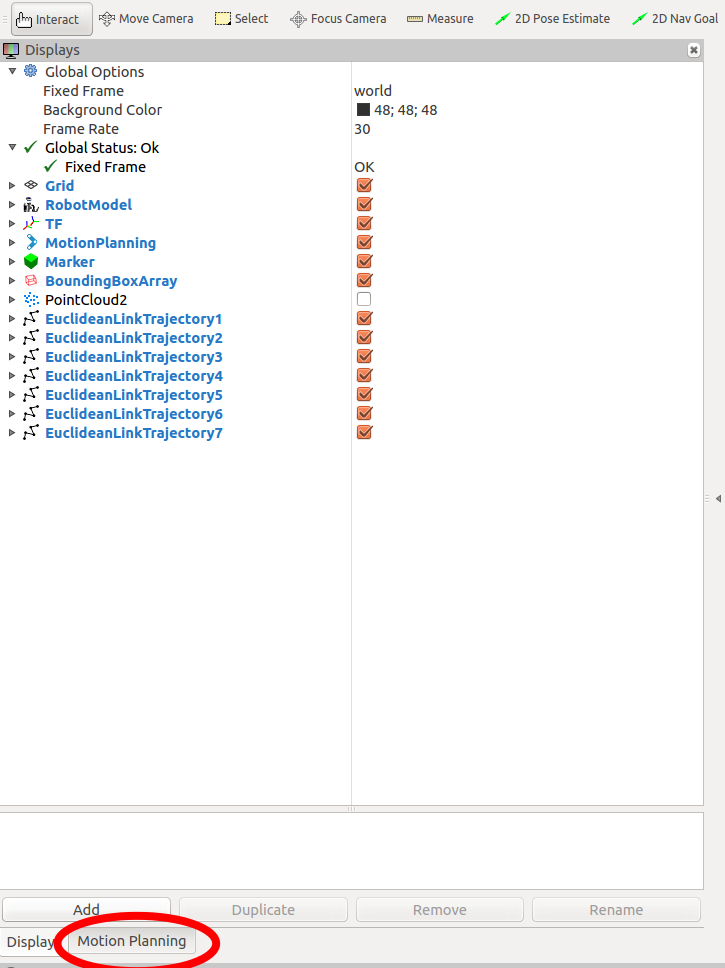
\includegraphics[scale=0.23]{images/motion_planning/gui_moving_procedure_1.png}
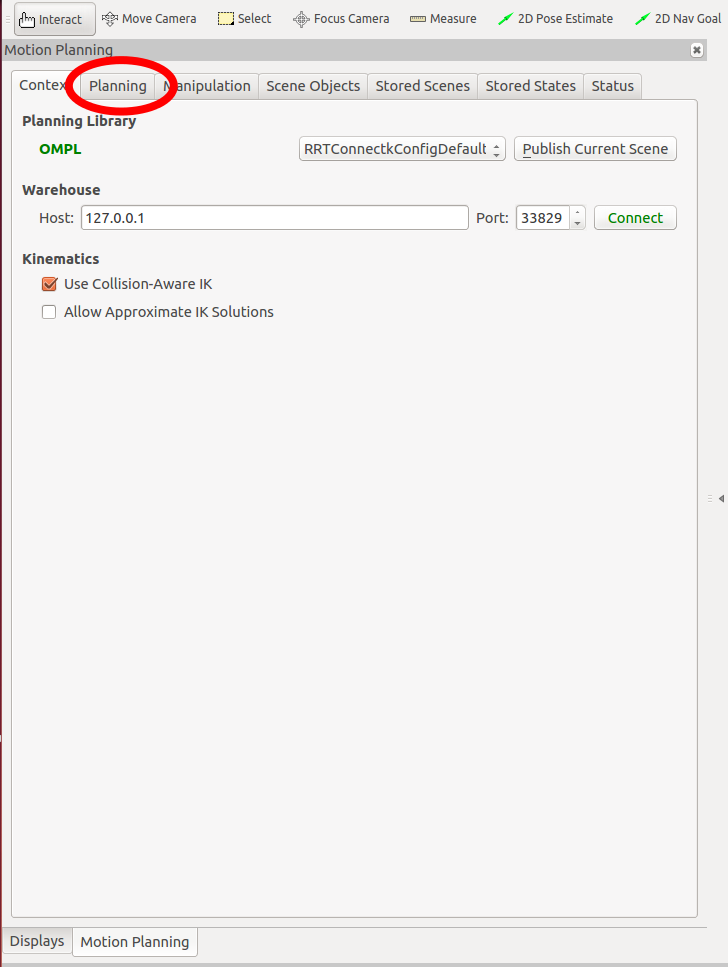
\includegraphics[scale=0.23]{images/motion_planning/gui_moving_procedure_2.png}
\centering
\caption{Clicking on \emph{motion planning}, then \emph{planning}.}
\label{fig:gui_procedure_1}
\end{figure}



\begin{figure}
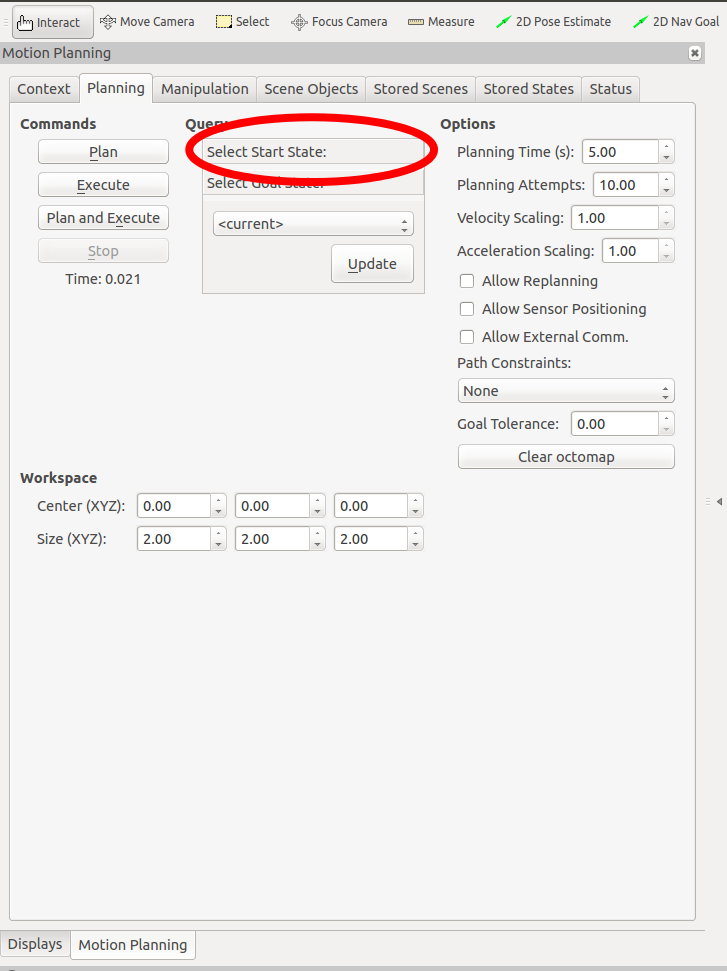
\includegraphics[scale=0.23]{images/motion_planning/gui_moving_procedure_3.png}
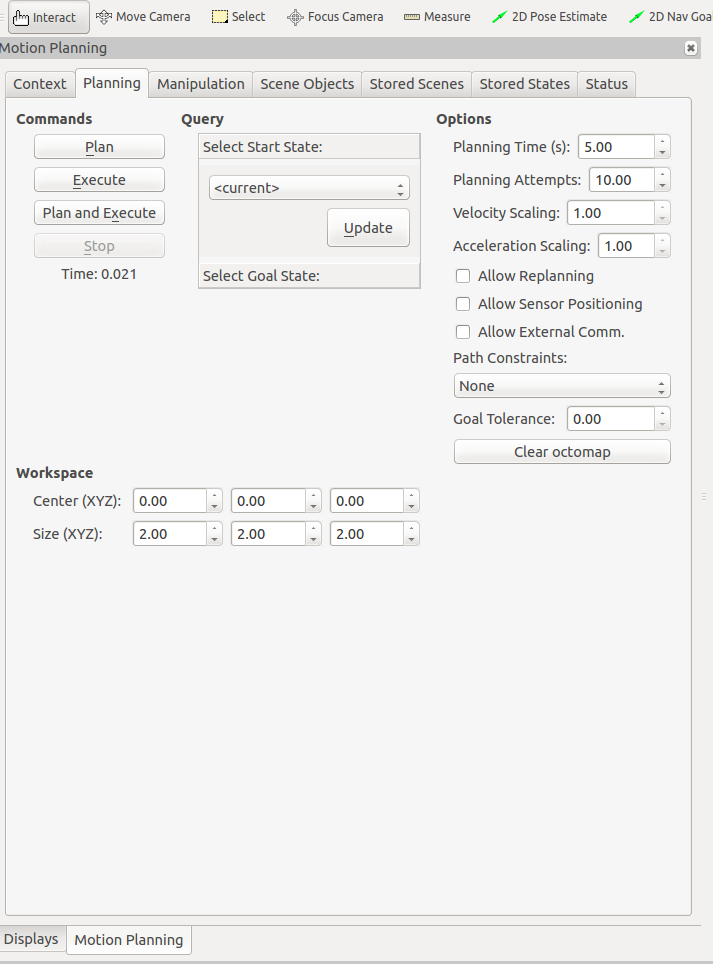
\includegraphics[scale=0.23]{images/motion_planning/gui_moving_procedure_4.png}
\centering
\caption{Clicking on \emph{select start state} and then the \emph{update} button.}
\label{fig:gui_procedure_2}
\end{figure}

\begin{figure}
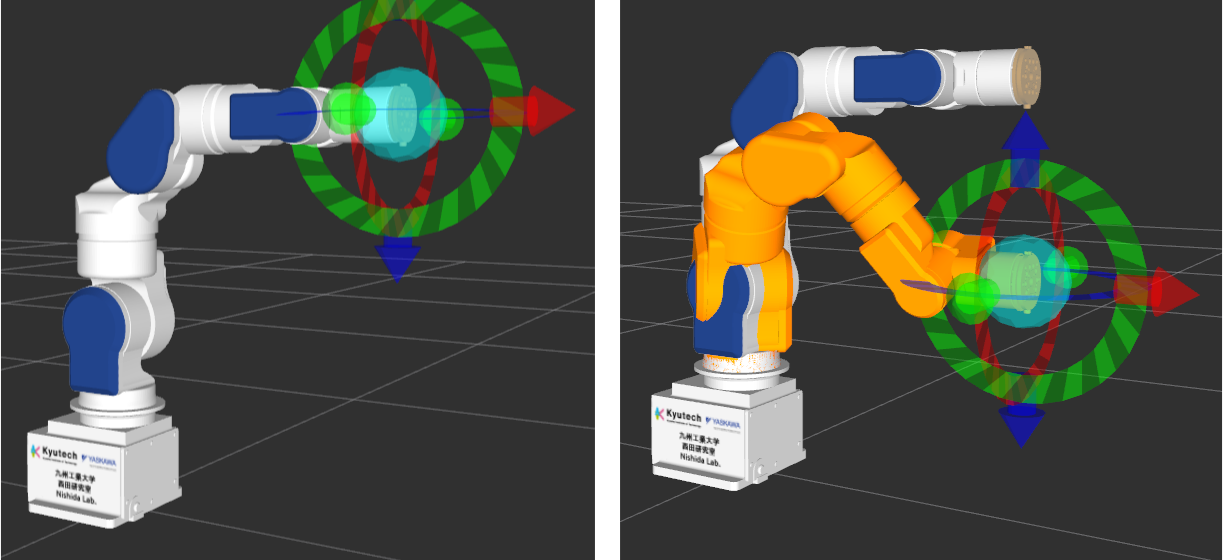
\includegraphics[scale=0.27]{images/motion_planning/gui_end_effector.png}
\centering
\caption{Changing the goal position by moving the end effector ball through the GUI.}
\label{fig:gui_end_effector}
\end{figure}

\section{Simple script}

In this section we review the script we used during chapter 2 to plan a motion between the home position to a specific position. We will describe the different parts of the code and in the following section we will build on this simple script. The script we used is the following one.

\lstinputlisting[language=c++,caption=moving.cpp]{code_files/motion_planning/moving.cpp}

The first important line is the creation of the object \emph{group}. Moveit will do the interface between the motion planners and the robot but it needs to be initialized to know what robot (or what part of the robot) to work on. In our case the whole parts of the robot will be used and it has been named \emph{arm} during the moveit initialization procedure, that is why we put it as an argument. Then we need to define the start and goal position for our planning problem. In this simple script we define the start position as the current position of the robot. Hence we need to get the current position of the robot with the method \emph{getCurrentState} of our object \emph{group}. For the goal position, we decided to define by ourself the exact position of all the joints of the robot and input it as the goal. To do it we first define a map data structure which will associate for each string (the name of the joint) a double (the joint value). The robot is a 7 degrees of freedom robot so there are 7 joints to give values to. Each joint has a name, you can see in figure \ref{fig:sia5_joints_name} their position with their name. The \emph{setJointValueTarget} method of the object \emph{group} is then the method to call to input the goal position from the previously created map. Eventually we need to call the \emph{plan} method from the \emph{group} object, but this method requires a \emph{Plan} object as argument to store the solution (or nothing if no plan is found). It should be noted that the plan method returns a boolean indicating if a solution has been found or not.

So this script was a really simple one to show the basis of a planning with the moveit library. In the following sections we will show how to add some obstacles in the environment, to change the motion planner and how to do a lot of planning.


\section{Moving to a pose}

Instead of specifying all the joint values it can be useful to just ask the end-effector to be at a defined pose (position and orientation). It is simple to do with moveit but be careful as your specified pose may not be possible to reach by the robot end-effector. The following code is the entire code to plan a motion to a pose goal.

\lstinputlisting[language=c++,caption=moving.cpp]{code_files/motion_planning/moving_to_pose.cpp}

You can see that the only part that changed was the goal state definition compared to the simple script. We first create a \emph{Pose} object and then set its attributes. Finally we inform moveit by using the \emph{setPoseTarget} method.